\documentclass[pdflatex, sn-nature, oneside]{sn-jnl}% Style for submissions to Nature Portfolio 

%%%% Standard Packages
\usepackage{graphicx}%
\usepackage{multirow}%
\usepackage{amsmath,amssymb,amsfonts}%
\usepackage{amsthm}%
\usepackage{mathrsfs}%
\usepackage[title]{appendix}%
\usepackage{xcolor}%
\usepackage{textcomp}%
\usepackage{manyfoot}%
\usepackage{booktabs}%
\usepackage{algorithm}%
\usepackage{algorithmicx}%
\usepackage{algpseudocode}%
\usepackage{listings}%
\usepackage{gensymb} %added by V. Van der Meersch
\usepackage{comment} %added by V. Van der Meersch

\raggedbottom
\unnumbered% uncomment this for unnumbered level heads

\begin{document}

\title[Article Title]{Contrasted hindcast performances demonstrate the need for more realistic models\par
\textbf{Extended Data} 
}

\author*[1]{\fnm{Victor} \sur{Van der Meersch}}\email{victor.vandermeersch@cefe.cnrs.fr}
\author[2]{\fnm{Edward} \sur{Armstrong}}
\author[3]{\fnm{Frédérik} \sur{Saltré}}
\author[1]{\fnm{Florent} \sur{Mouillot}}
\author[4]{\fnm{Anne} \sur{Duputié}}
\author[5]{\fnm{Cristophe} \sur{Randin}}
\author[6]{\fnm{Hendrik} \sur{Davi}}
\author[1]{\fnm{Isabelle} \sur{Chuine}}

\affil[1]{\orgdiv{CEFE}, \orgname{Université de Montpellier, CNRS, EPHE, IRD}, \orgaddress{\city{Montpellier}, \country{France}}}
\affil[2]{\orgdiv{Dept. of Geosciences and Geography}, \orgname{University of Helsinki}, \orgaddress{\city{Helsinki}, \country{Finland}}}
\affil[3]{\orgdiv{Global Ecology}, \orgname{College of Science and Engineering, Flinders University}, \orgaddress{\city{Adelaide}, \country{Australia}}}
\affil[4]{\orgdiv{UMR 8198-EEP-Evo-Eco-Paleo}, \orgname{Université de Lille, CNRS}, \orgaddress{\city{Lille}, \country{France}}}
\affil[5]{\orgdiv{Dept. of Ecology and Evolution}, \orgname{Univ. Lausanne}, \orgaddress{\city{Lausanne}, \country{Switzerland}}}
\affil[6]{\orgdiv{URFM}, \orgname{INRAE}, \orgaddress{\city{Avignon}, \country{France}}}

\maketitle

\newpage

\begin{figure}
\hspace*{-0.5in}
\centering
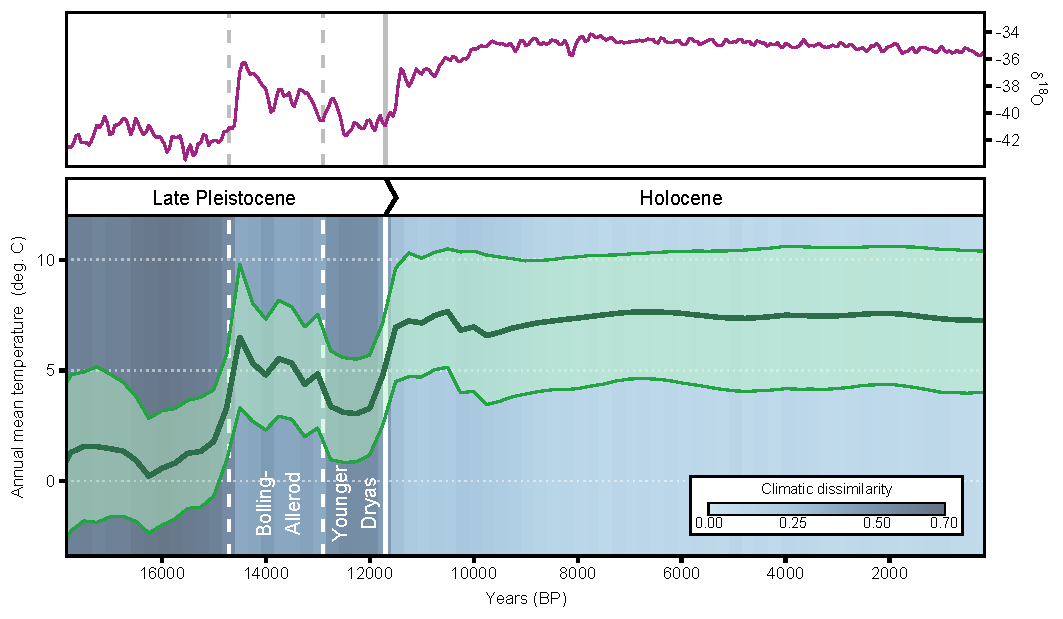
\includegraphics{climate_overview-1.pdf}
\caption{\textbf{Chronology of past climate across the Late Pleistocene and the Holocene.} Upper panel shows the evolution of North Greenland Ice-Core Project (NGRIP) oxygen isotope 18 values (permille) as 50 year mean values \cite{Andersen2004}. Lower panel shows the average annual temperature across Europe, from HadCM3B simulations \cite{Armstrong2019}. Shaded area  represents 25\% and 75\% quantiles. Blue background represents the level of climatic dissimilarity (see Methods).}
\end{figure}

\begin{figure}
\hspace*{-0.5in}
\centering
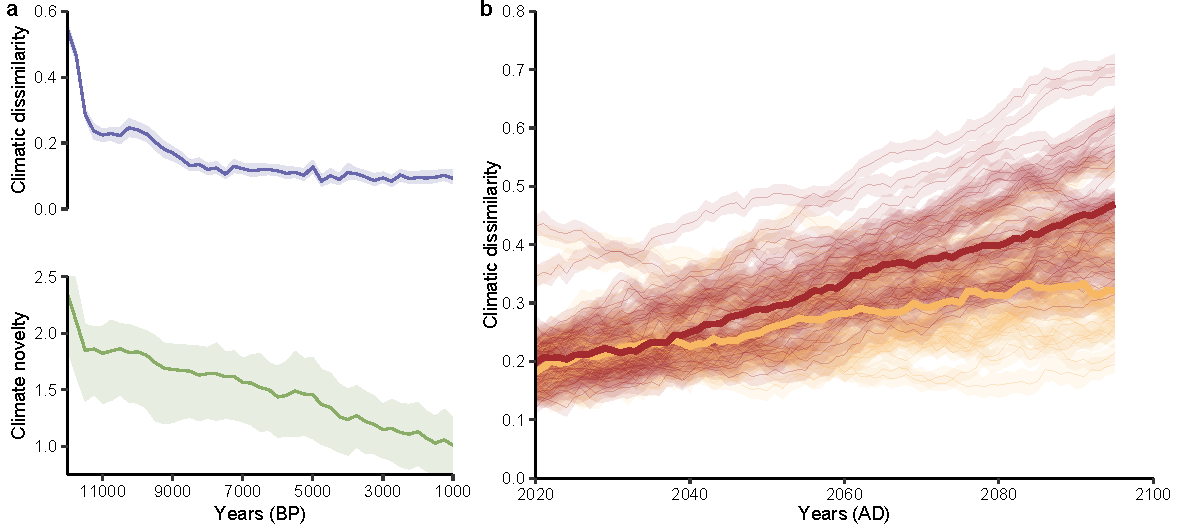
\includegraphics{climatic_dissimilarity_and_distance-1.pdf}
\caption{\textbf{(a)} Comparison of climatic dissimilarity as calculated in this paper and climate novelty calculated following \cite{Burke2019} \textbf{(b)} Evolution of future climatic dissimilarity, across the different GCM simulations. Yellow and red correspond to SSP245 and SSP585 scenarios. }
\end{figure}

\begin{figure}
\hspace*{-0.7in}
\centering
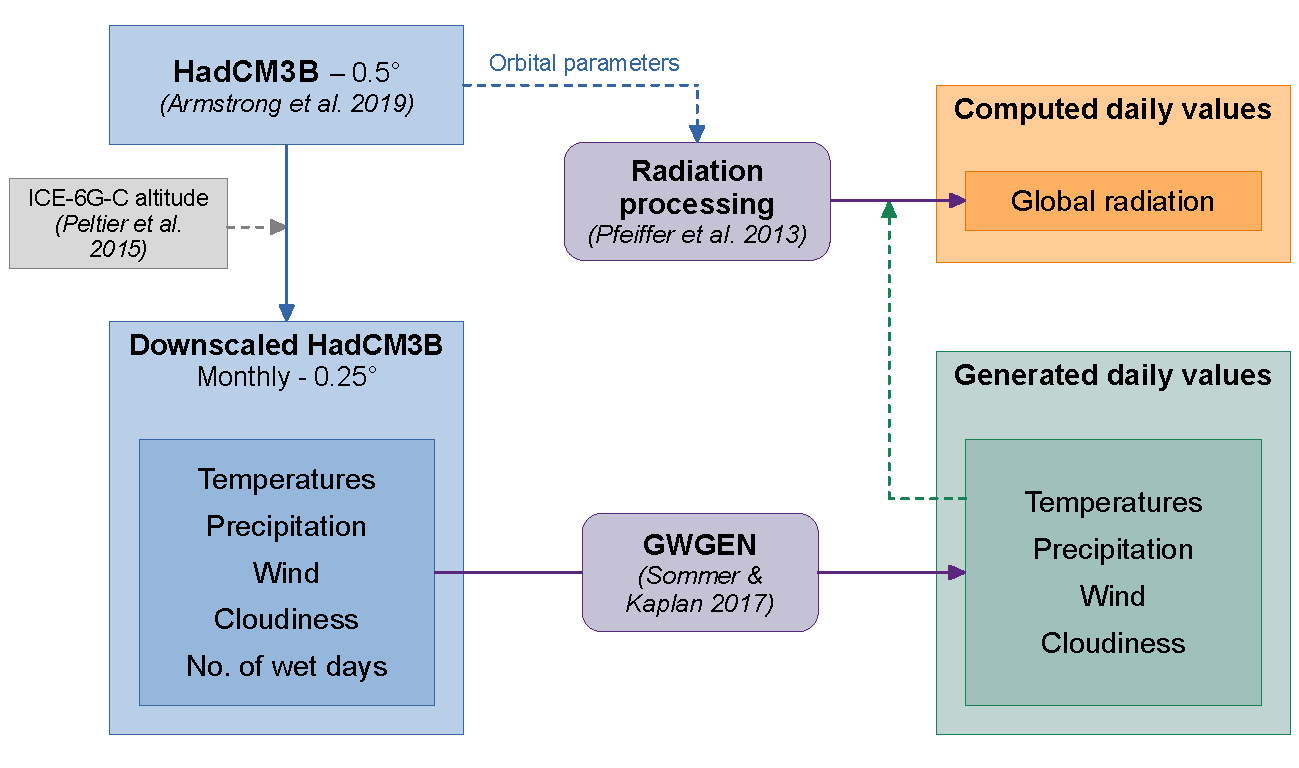
\includegraphics[scale=0.85]{paleoclimate_processing.pdf}
\caption{\textbf{Paleoclimate processing framework used in this study.} Monthly simulations come from HadCM3B-M2.1 coupled general circulation model \cite{Armstrong2019}. Daily data were generated using the weather generator GWGEN \cite{Sommer2017}. Daily global radiation were simulated as in LPJ-LMfire global model \cite{Pfeiffer2013}.}
\end{figure}

\begin{figure}
\hspace*{-0.3in}
\centering
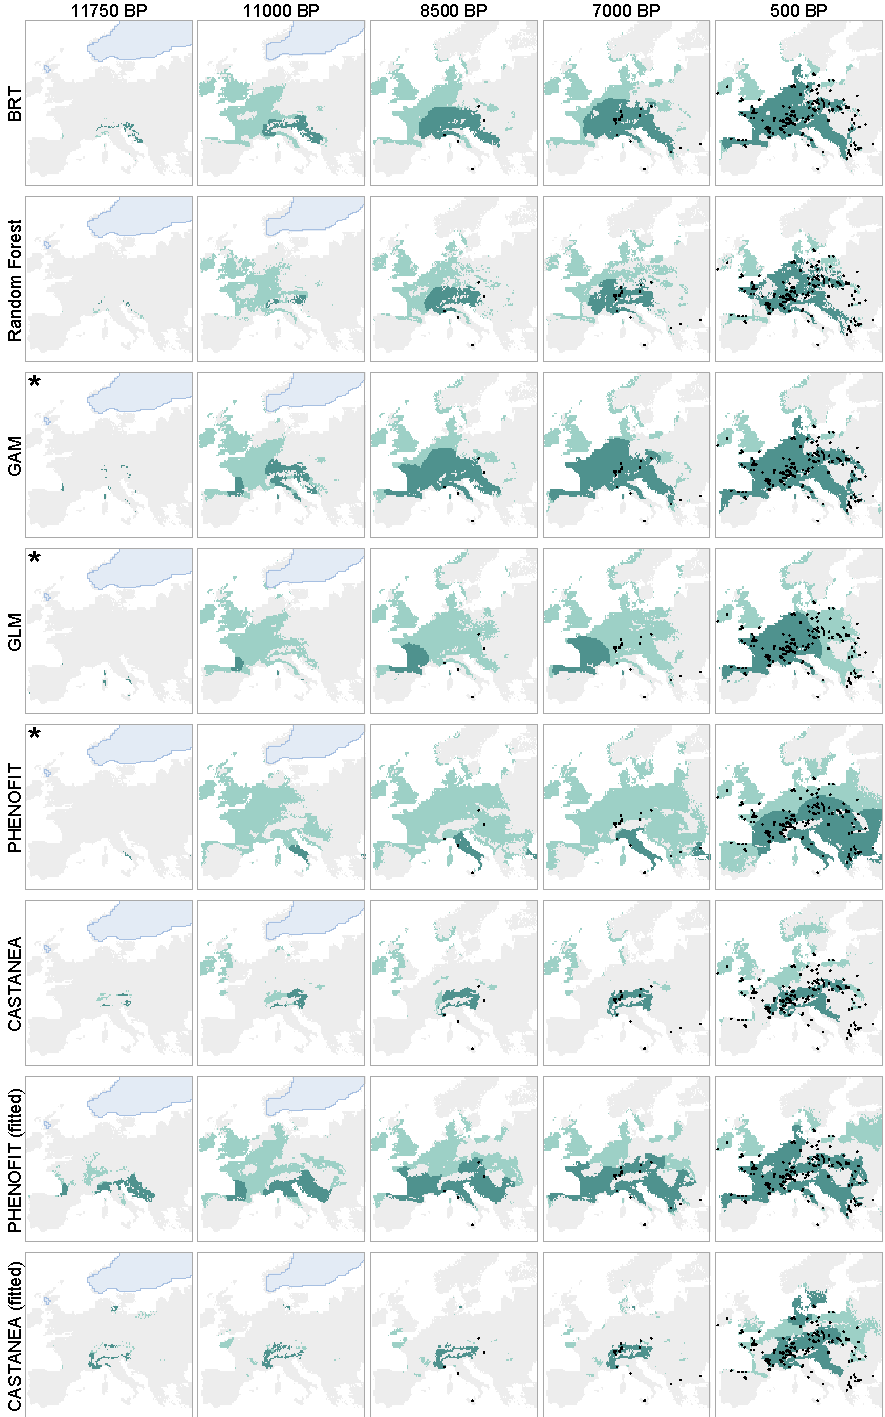
\includegraphics{fagus_simulations-1.pdf}
\caption{Same caption as Fig. 2 in the main text, for beech.}
\end{figure}

\begin{figure}
\hspace*{-.3in}
\centering
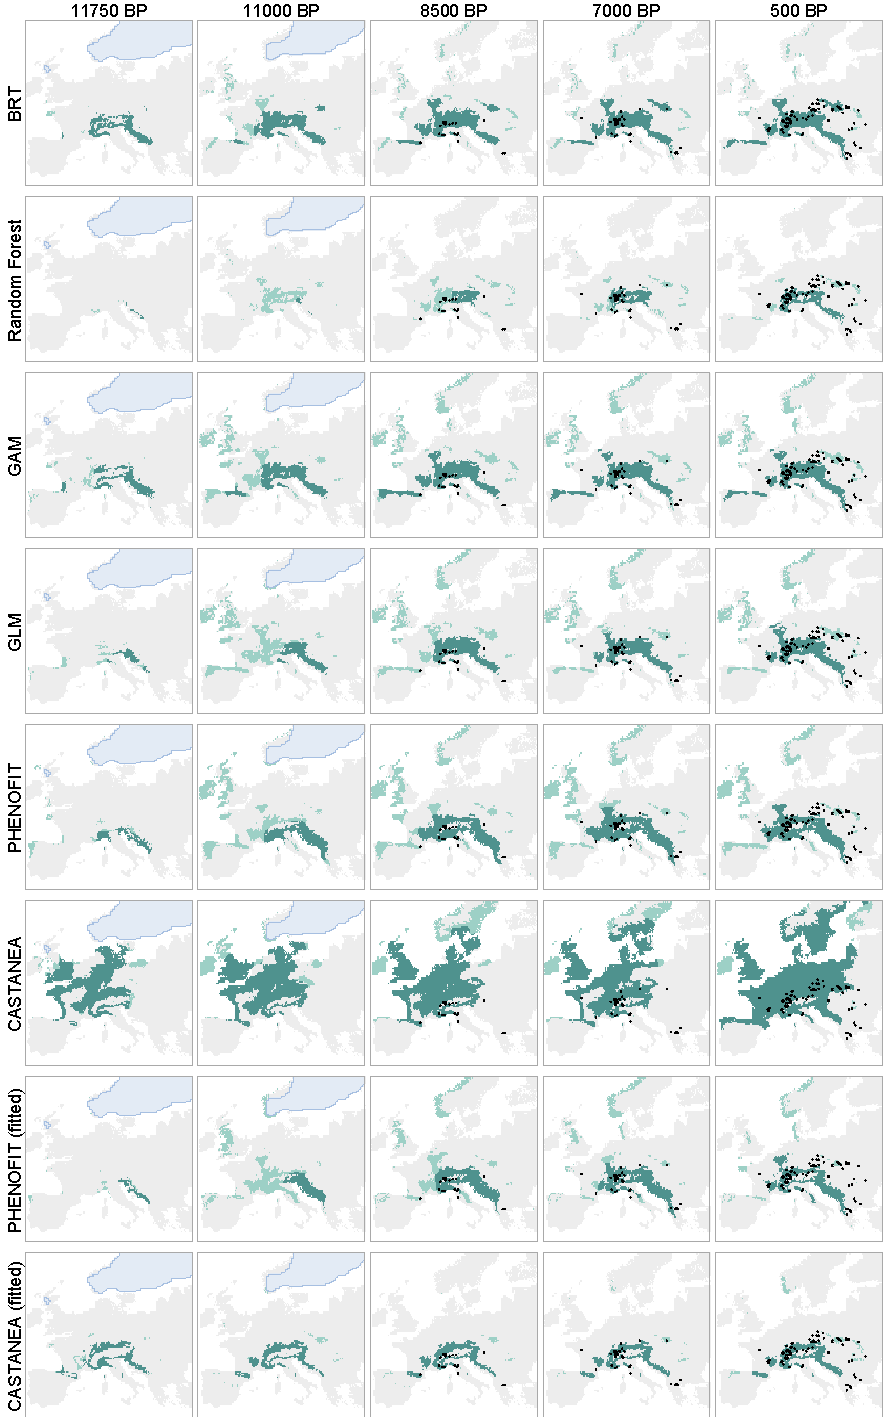
\includegraphics{abies_simulations-1.pdf}
\caption{Same caption as Fig. 2 in the main text, for fir.}
\end{figure}

\begin{figure}
\hspace*{-.3in}
\centering
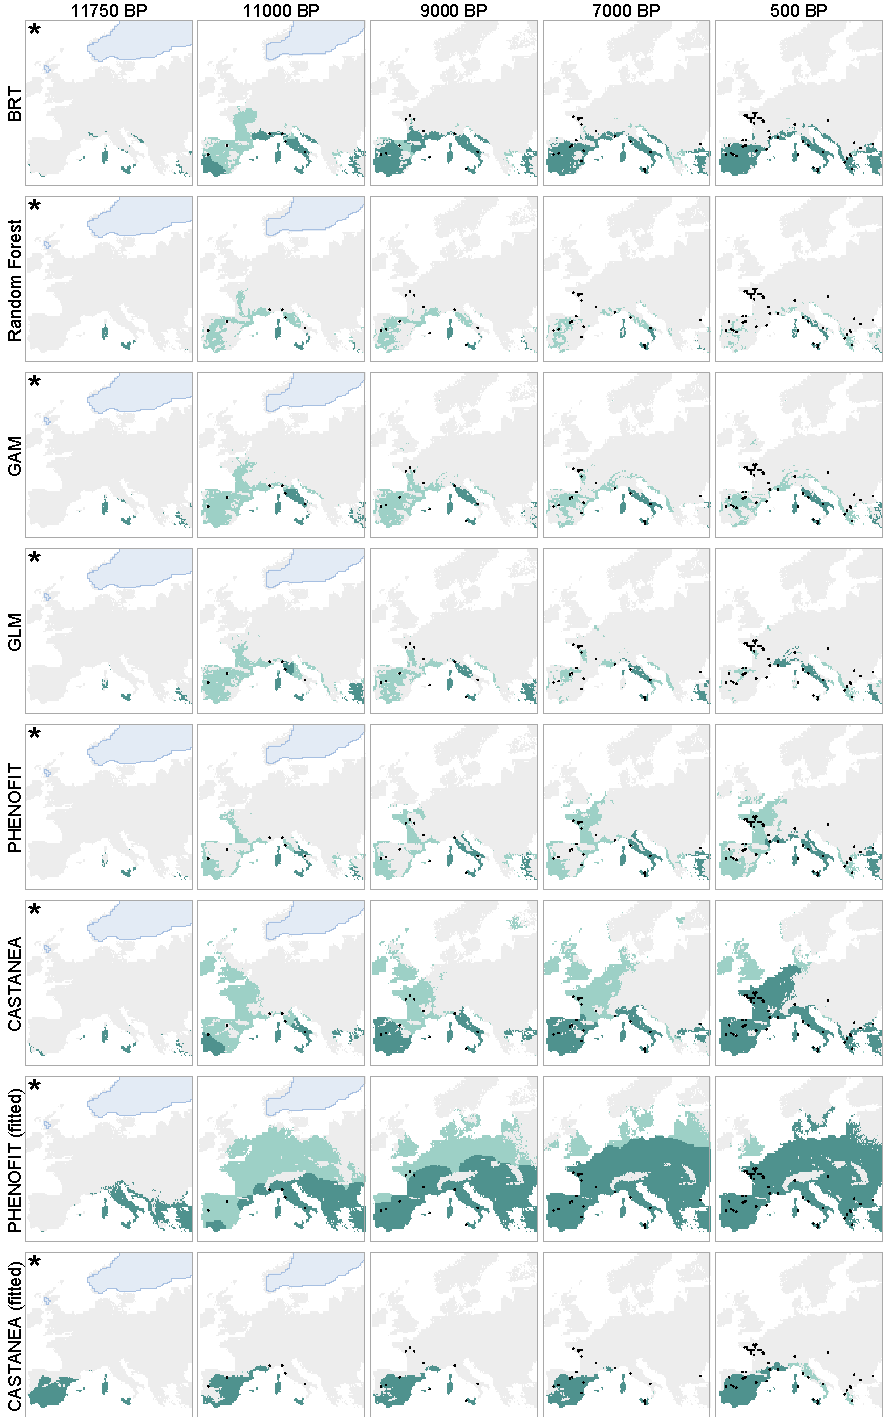
\includegraphics{quercusevergreen_simulations-1.pdf}
\caption{Same caption as Fig. 2 in the main text, for evergreen oak.}
\end{figure}

\begin{figure}
\hspace*{-0.4in}
\centering
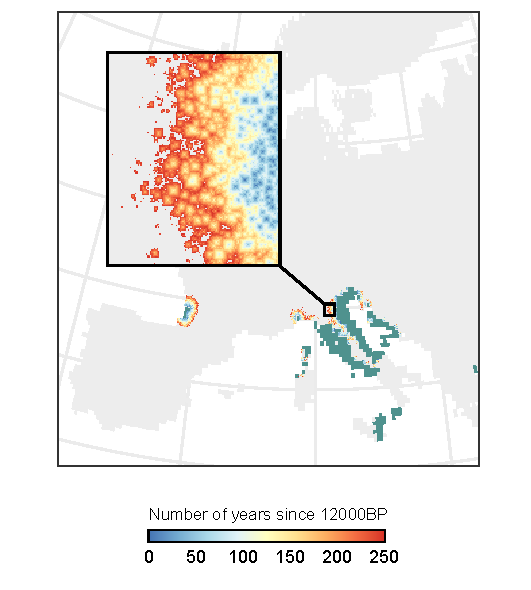
\includegraphics{migration_process-1.pdf}
\caption{Illustration of the first 250 years of deciduous oak migration process, with PHENOFIT fitted model. Dark green area represents migration starting points at 12000 BP.}
\end{figure}

\begin{figure}
\hspace*{-0.4in}
\centering
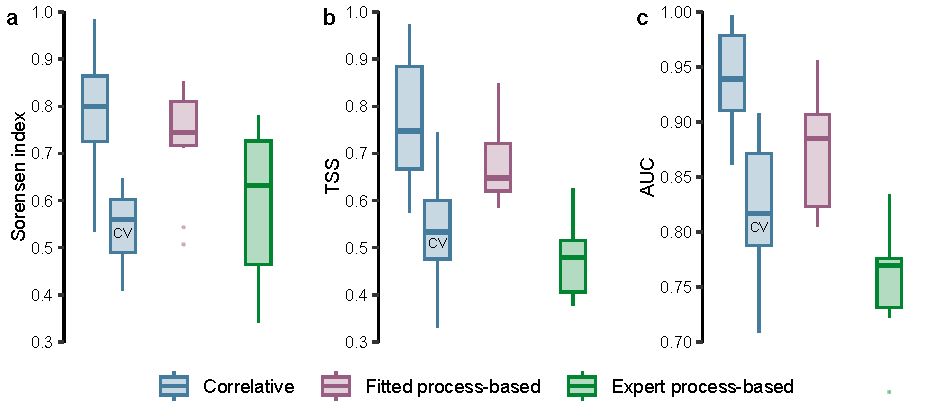
\includegraphics{historical_perf-1.pdf}
\caption{\textbf{Model performance in historical conditions.} . ”CV” stands for ”cross-validation”, when
correlative extrapolation errors were assessed using a block cross-validation method.}
\end{figure}

\begin{figure}
\hspace*{-0.8in}
\centering
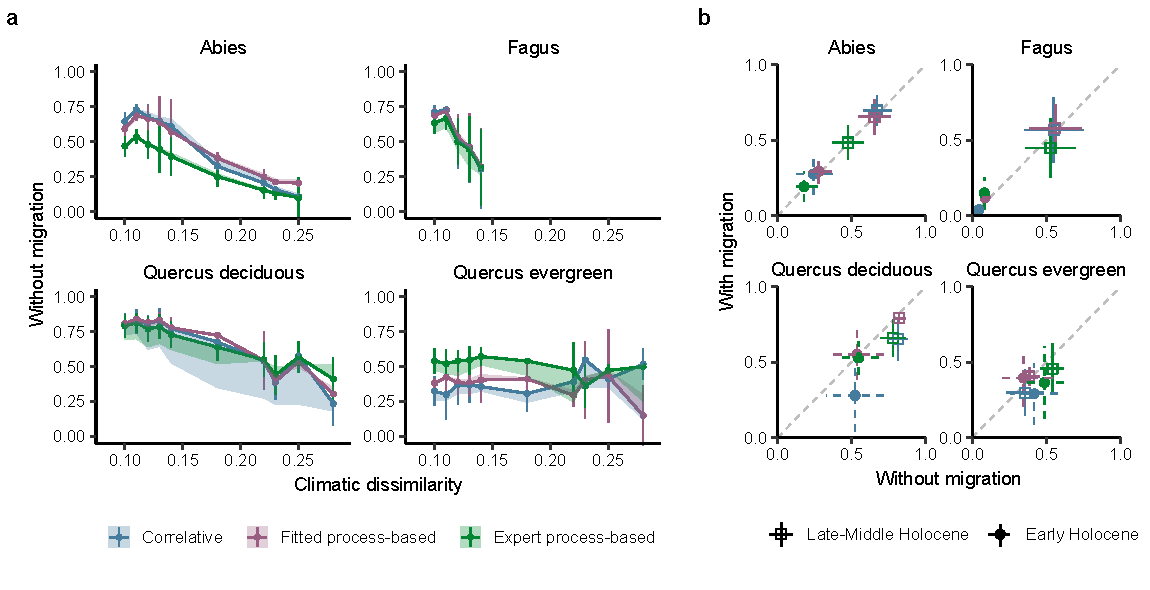
\includegraphics{performance_perspeciesmigration-1.pdf}
\caption{\textbf{Impacts of migration on model performance, per species.} \textbf{(a)} Evolution of performance against climatic dissimilarity. Lines and points represent model performance without migration, shaded areas show performance evolution when simulating migration. Panel \textbf{(b)} displays model performance with and without migration, for Late-Middle and Early Holocene.}
\end{figure}

\begin{figure}
\hspace*{-0.6in}
\centering
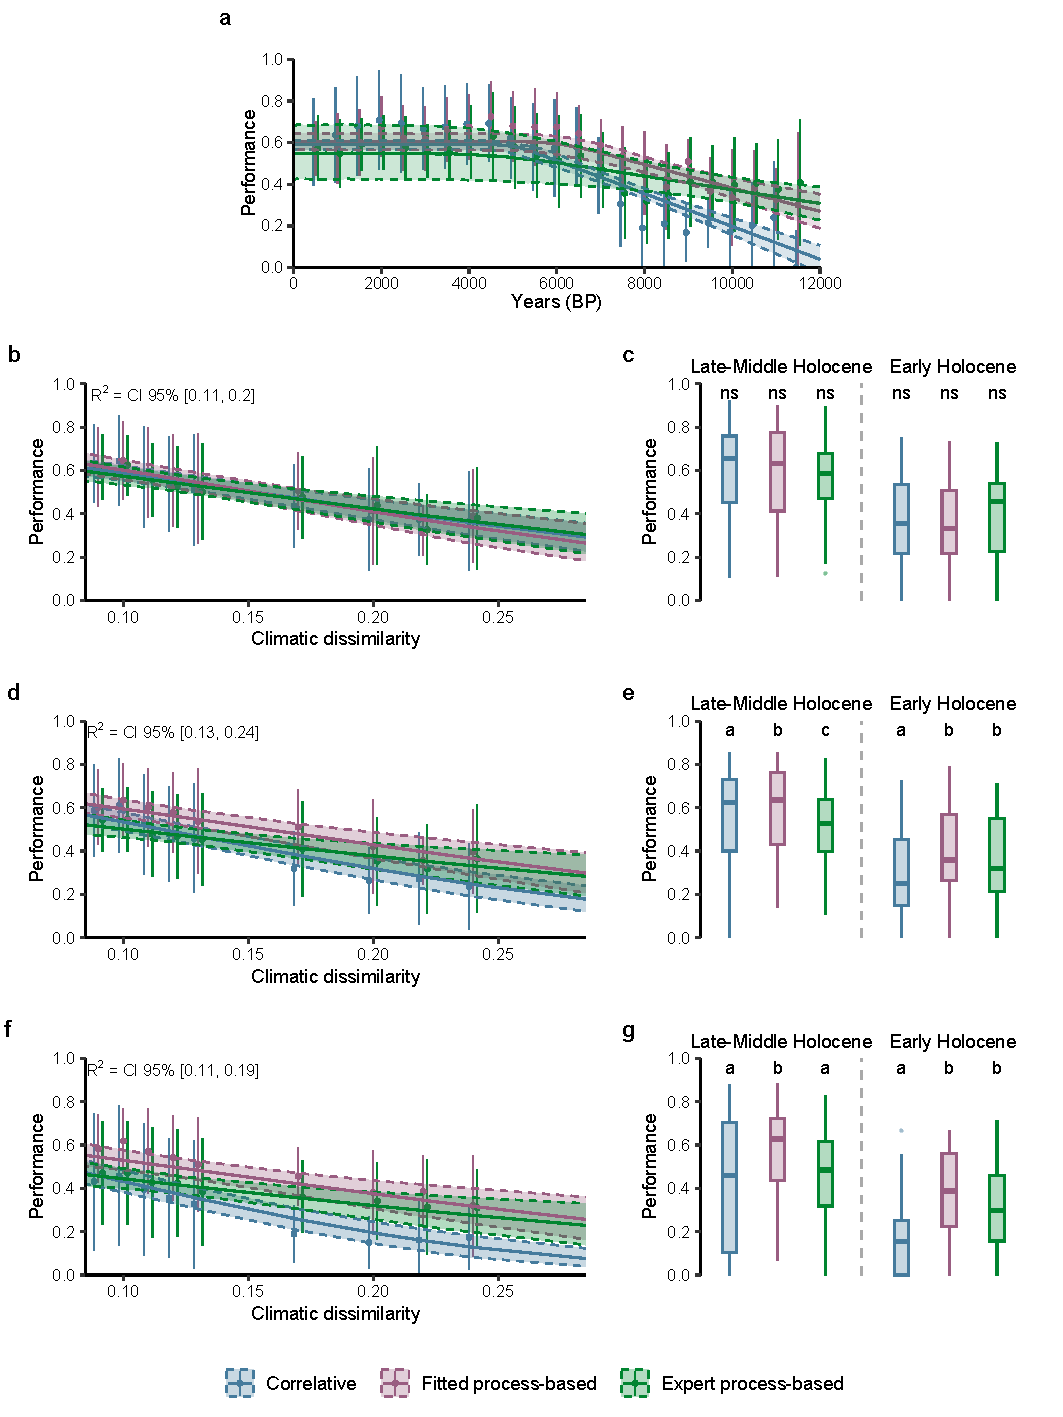
\includegraphics{past_performance_differentstarts-1.pdf}
\caption{\textbf{Performance of correlative models, fitted process-based models (inverse calibration using occurrence data) and expert process-based models (classical calibration).}
\textbf{(a)} Lines are linear-plateau regressions, which follow two phases (a flat plateau and a linear response). Shaded areas represents 2.5\% and 97.5\% confidence intervals, calculated with the R package \emph{propagate} \cite{Spiess2018} by using  first and second-order Taylor expansion and Monte Carlo simulations.
\textbf{(b,d,f)} Bayesian beta regression of model performance (Sørensen index) against climatic dissimilarity, and \textbf{(c,e,g)} difference in performance across models. The grouping letters represent the multiple comparisons with pairwise Conover-Iman tests.
\textbf{(b,c)} Models without migration, \textbf{(d,e)} models with all migration starting points at 11750 BP, \textbf{(f,g)} models with all migration starting points at 12000 BP.}
\end{figure}

\clearpage

\bibliography{robustness_bibliography} 

\end{document}
